\item \textbf{{[}ALVL/9597/2018/P2/Q1{]} }

A mobile phone company has an option for Pay As You Go usage. Customers
have to purchase credit in advance. The credit is used to pay for
texts, calls and data. Customers can buy additional credit at any
time. 

The company requires software to allow their Pay As You Go customers
to do the following tasks online: 
\begin{itemize}
\item check credit balance 
\item check data usage 
\item check call usage 
\item pay for credit 
\end{itemize}
A software company was employed to put together a project team to
produce the software. 
\begin{enumerate}
\item State \textbf{three} members of the project team. Describe the role
of each of these members. \hfill{}{[}6{]}
\item The initial phase of the system development cycle required that a
specification be created for the system. 
\begin{enumerate}
\item State \textbf{two} techniques that could have been used to gather
the information for this specification. \hfill{} {[}2{]}
\item Explain how each technique would have been used in this project. \hfill{}
{[}4{]}
\end{enumerate}
\item The specification is a detailed report.

Describe \textbf{two} sections of this report. \hfill{}{[}4{]}
\item The software could have been designed using different techniques. 
\begin{enumerate}
\item Name \textbf{and} describe \textbf{two} design techniques that may
have been used. \hfill{} {[}4{]}
\item Explain why it is important for each member of the design team to
use the same technique. \hfill{} {[}2{]}
\item A customer's mobile phone number needs to be validated on entry. 

Draw a flowchart to represent an algorithm for this validation. \hfill{}
{[}4{]}
\end{enumerate}
\item (e) The work to implement the new software needs to be managed. The
following Program Evaluation and Review Technique (PERT) chart is
used as a management tool. 

\texttt{A} --- Specification 

\texttt{B} --- Analysis 

\texttt{C} --- Design of software 

\texttt{D} --- Design of Interface 

\texttt{E} --- Documentation 

\texttt{F}--- Implementation 

\texttt{G} --- Testing 

\texttt{H} --- Acceptance testing

\texttt{I} --- Hand over to phone company 

Time is measured in weeks. 
\begin{center}
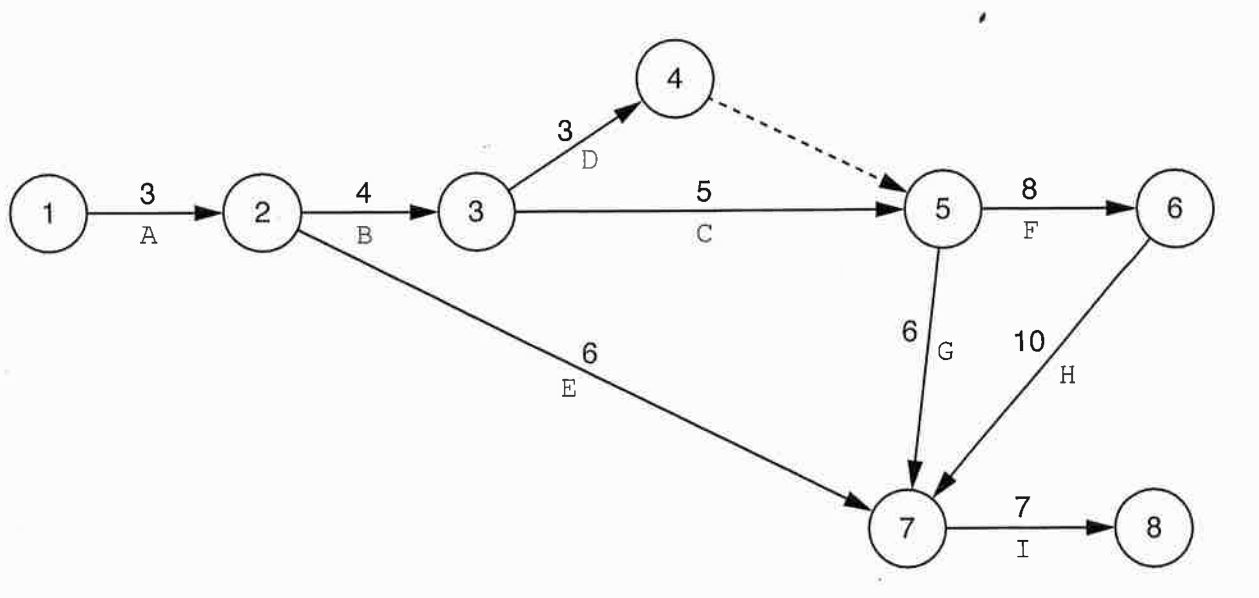
\includegraphics[width=0.5\paperwidth]{C:/Users/Admin/Desktop/Github/question_bank/LyX/static/img/9597-ALVL-2018-P2-Q1}
\par\end{center}
\begin{enumerate}
\item State the critical path for the given activities \texttt{A} to \texttt{I}.
\hfill{}{[}2{]}
\item Calculate the minimum time these activities will take. \hfill{}{[}1{]}
\item The member of the project team who worked on activity 0 fold the project
manager he could not start work until one week after the scheduled
start date. 

Explain any impact this would have on the completion date of the project.\hfill{}
{[}3{]}
\end{enumerate}
\item The software is intended for use on hand-held devices. 

Describe \textbf{two} ways that users can keep their data secure on
these devices.\hfill{} {[}4{]}
\item A member of the project team had the task of ensuring that social
and ethical issues were considered. 

Describe \textbf{one} example of each of these Issues that this member
of the team might have considered. \hfill{}{[}4{]}
\end{enumerate}